\documentclass[border=18pt,tikz]{standalone}
\usepackage{amsmath,amssymb,bm}
\usetikzlibrary{arrows.meta,positioning,calc,decorations.pathreplacing,fit,backgrounds}

% ============================================================
%  arch_common.tex  --  shared TikZ styles for MTP-PINN figures
%  All fonts bumped to \large; inner sep generous; no overlaps.
% ============================================================
\newcommand{\ArchBlockFont}{\large}
\newcommand{\ArchPhaseHdr}{\large\bfseries\color{black!80}}

%% --- Colour palette --------------------------------------------------------
\definecolor{KinFill}{RGB}{224,247,250}
\definecolor{KinDraw}{RGB}{0,131,143}
\definecolor{PhyFill}{RGB}{255,243,224}
\definecolor{PhyDraw}{RGB}{230,81,0}
\definecolor{NrmFill}{RGB}{243,229,245}
\definecolor{NrmDraw}{RGB}{106,27,154}
\definecolor{CatFill}{RGB}{255,249,196}
\definecolor{CatDraw}{RGB}{245,127,23}
\definecolor{MlpFill}{RGB}{227,242,253}
\definecolor{MlpDraw}{RGB}{21,101,192}
\definecolor{TanhFill}{RGB}{237,231,246}
\definecolor{TanhDraw}{RGB}{123,31,162}
\definecolor{AddFill}{RGB}{241,248,233}
\definecolor{AddDraw}{RGB}{85,139,47}
\definecolor{OutFill}{RGB}{232,245,233}
\definecolor{OutDraw}{RGB}{46,125,50}
\definecolor{LossFill}{RGB}{255,235,238}
\definecolor{LossDraw}{RGB}{183,28,28}
\definecolor{PhysBpFill}{RGB}{255,248,225}
\definecolor{PhysBpDraw}{RGB}{249,168,37}
\definecolor{NoteFill}{RGB}{245,245,245}
\definecolor{NoteDraw}{RGB}{100,100,100}

%% --- TikZ styles -----------------------------------------------------------
\tikzset{
  every node/.style={align=center},
  line cap=round,
  %% base block
  blk/.style={
    draw=gray!55,
    line width=1.6pt,
    rounded corners=6pt,
    inner sep=14pt,
  },
  %% domain blocks
  kinBlk/.style={
    blk, fill=KinFill, draw=KinDraw,
    minimum width=4.2cm,
    font=\ArchBlockFont,
  },
  phyBlk/.style={
    blk, fill=PhyFill, draw=PhyDraw,
    minimum width=5.8cm,
    font=\ArchBlockFont,
  },
  nrmBlk/.style={
    blk, fill=NrmFill, draw=NrmDraw,
    minimum width=4.0cm,
    font=\ArchBlockFont,
  },
  catBlk/.style={
    blk, fill=CatFill, draw=CatDraw,
    minimum width=2.2cm,
    font=\ArchBlockFont,
  },
  mlpBlk/.style={
    blk, fill=MlpFill, draw=MlpDraw,
    minimum width=3.6cm,
    font=\ArchBlockFont,
  },
  fcBlk/.style={
    blk, fill=MlpFill, draw=MlpDraw,
    minimum width=3.4cm,
    font=\ArchBlockFont,
  },
  tanhBlk/.style={
    blk, fill=TanhFill, draw=TanhDraw,
    minimum width=3.4cm,
    font=\ArchBlockFont,
  },
  outBlk/.style={
    blk, fill=OutFill, draw=OutDraw,
    minimum width=3.4cm,
    font=\ArchBlockFont,
  },
  addBlk/.style={
    circle,
    draw=AddDraw,
    fill=AddFill,
    line width=1.5pt,
    minimum size=1.4cm,
    font=\LARGE\bfseries,
  },
  gtBlk/.style={
    blk, draw=NoteDraw, fill=NoteFill,
    line width=1.2pt,
    rounded corners=5pt,
    inner sep=12pt,
    font=\ArchBlockFont,
    minimum width=3.2cm,
  },
  lossBlk/.style={
    blk, fill=LossFill, draw=LossDraw,
    line width=1.4pt,
    inner sep=16pt,
    font=\ArchBlockFont,
  },
  bpBlk/.style={
    blk, fill=PhysBpFill, draw=PhysBpDraw,
    inner sep=10pt,
    font=\ArchBlockFont,
  },
  %% arrows
  arr/.style={
    -{Stealth[length=11pt,width=9pt]},
    line width=1.8pt,
    black!80,
  },
  darr/.style={
    -{Stealth[length=9pt,width=7.5pt]},
    line width=1.5pt,
    dashed,
    dash pattern=on 5pt off 3pt,
    black!50,
  },
  bparr/.style={
    -{Stealth[length=11pt,width=9pt]},
    line width=1.8pt,
    PhyDraw!90,
    rounded corners=4pt,
  },
  %% edge labels
  dim/.style={
    font=\large,
    fill=white,
    inner sep=3pt,
    above=1pt,
    midway,
    sloped=false,
  },
  diml/.style={
    font=\large,
    fill=white,
    inner sep=3pt,
    below=1pt,
    midway,
  },
  phaseHdr/.style={
    font=\ArchPhaseHdr,
    inner sep=0pt,
    outer sep=0pt,
    anchor=south west,
  },
}


\def\BH{5.2cm}
\def\IH{2.3cm}

\begin{document}
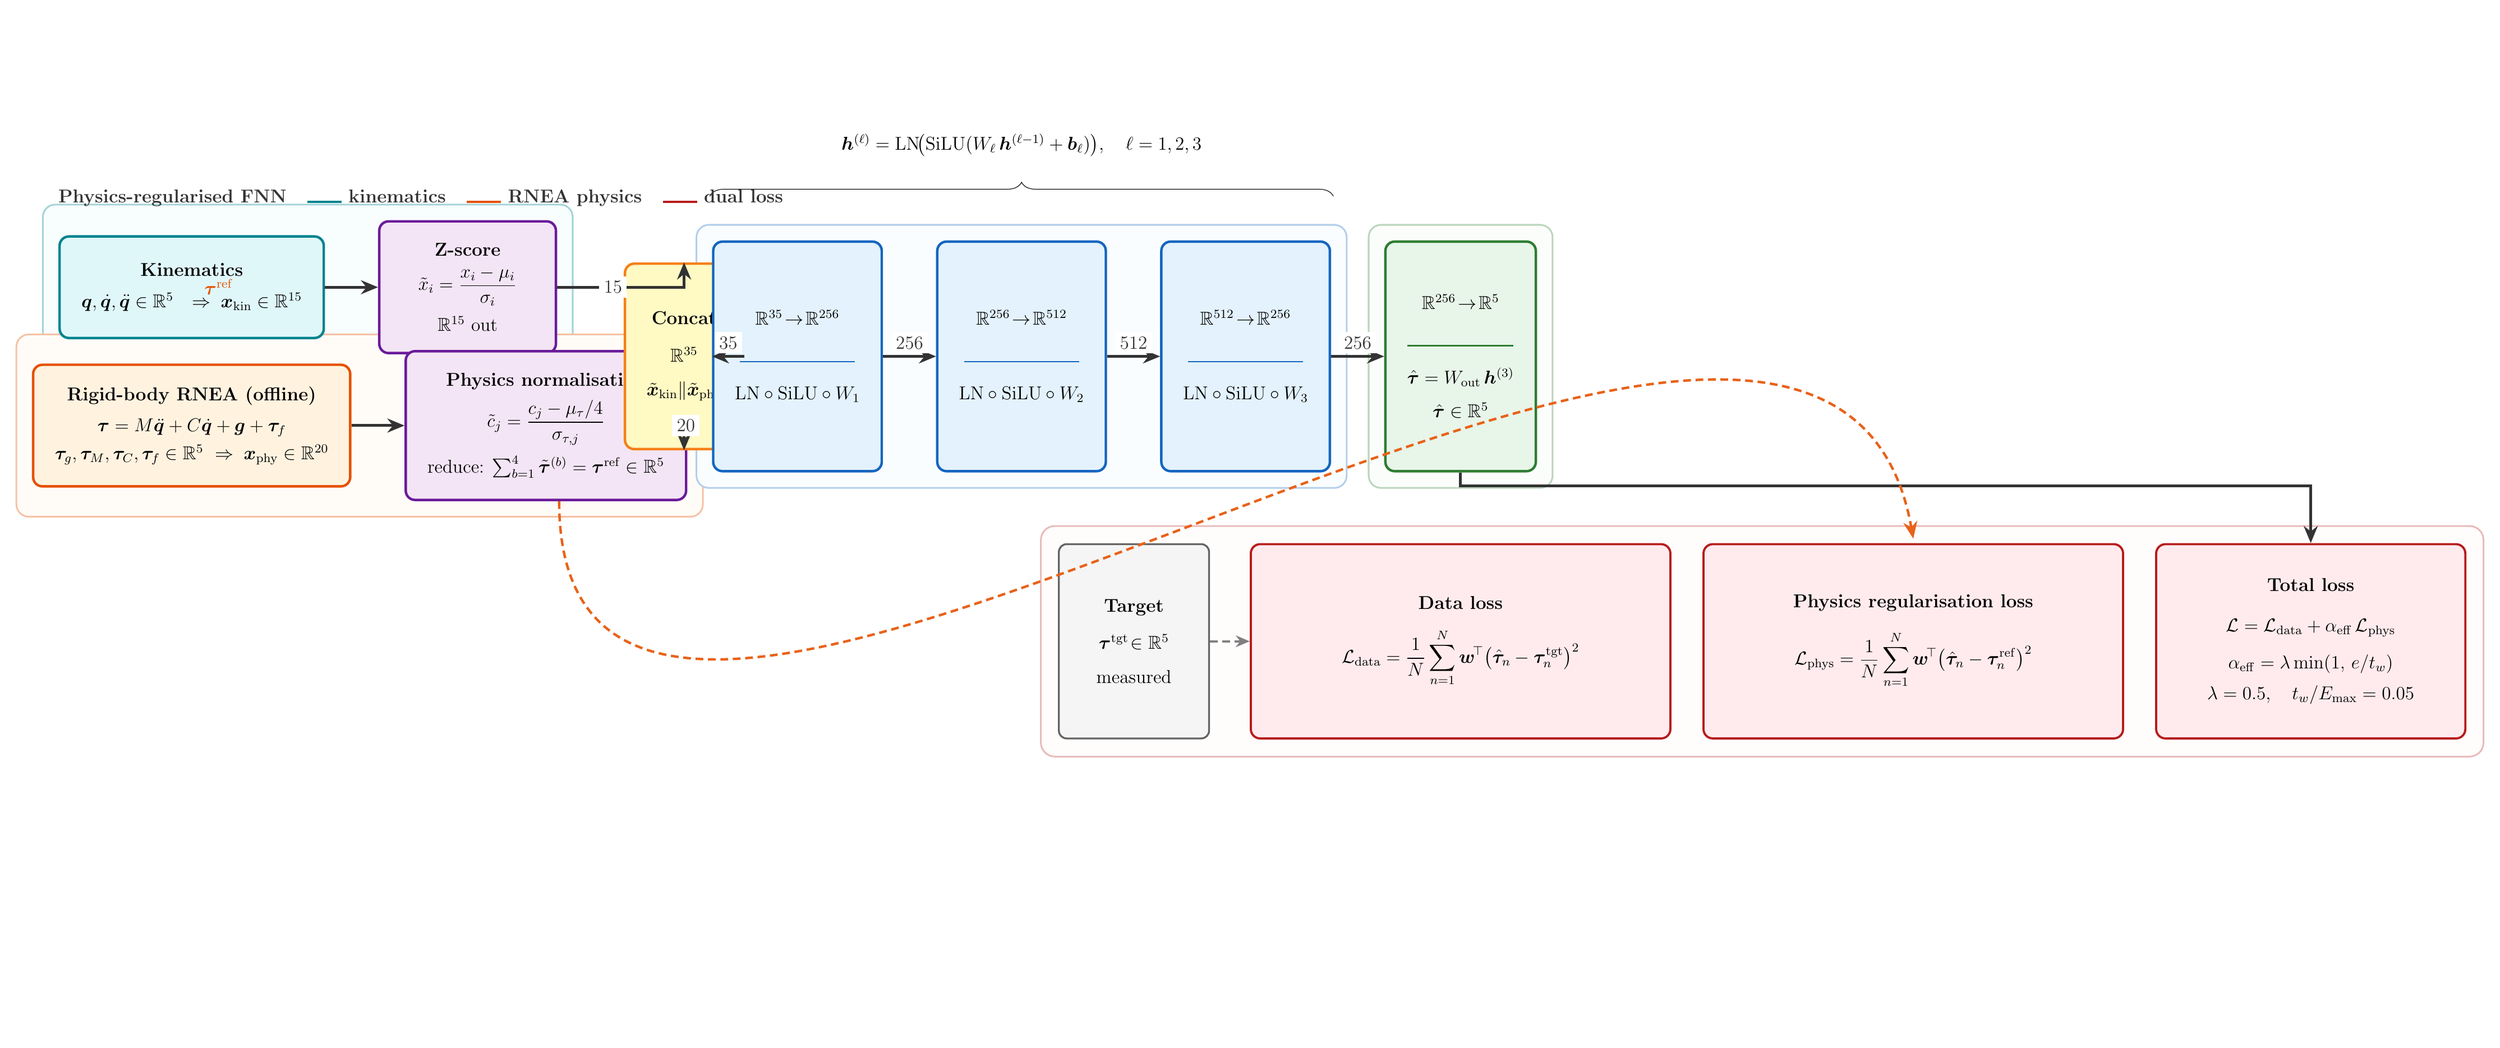
\begin{tikzpicture}[node distance=1.2cm]

%%─────────────────────────────────────────────────────────────────────────────
%% DESIGN  (left→right, all on one baseline)
%%─────────────────────────────────────────────────────────────────────────────

%%═══════════════════════════════ INPUT COLUMN ════════════════════════════════
%% Kinematics input (top half)
\node[kinBlk,
      minimum height=\IH, minimum width=4.4cm]
  (KINPUT) at (0,0) {%
  \textbf{Kinematics}\\[6pt]
  $\bm{q},\dot{\bm{q}},\ddot{\bm{q}}\in\mathbb{R}^{5}$\quad
  $\Rightarrow\;\bm{x}_{\mathrm{kin}}\in\mathbb{R}^{15}$
};

%% Physics input (bottom half, tight gap)
\node[phyBlk,
      minimum height=\IH, minimum width=5.8cm,
      below=0.55cm of KINPUT.south, anchor=north]
  (PINPUT) {%
  \textbf{Rigid-body RNEA (offline)}\\[6pt]
  $\bm{\tau}=M\ddot{\bm{q}}+C\dot{\bm{q}}+\bm{g}+\bm{\tau}_{f}$\\[4pt]
  {\large $\bm{\tau}_{g},\bm{\tau}_{M},\bm{\tau}_{C},\bm{\tau}_{f}\in\mathbb{R}^{5}$
    $\;\Rightarrow\;\bm{x}_{\mathrm{phy}}\in\mathbb{R}^{20}$}
};

%%═══════════════════════════════ NORM COLUMN ═════════════════════════════════
\node[nrmBlk,
      minimum height=\IH, minimum width=4.0cm,
      right=1.2cm of KINPUT]
  (KNORM) {%
  \textbf{Z-score}\\[6pt]
  $\tilde{x}_{i}=\dfrac{x_{i}-\mu_{i}}{\sigma_{i}}$\\[6pt]
  $\mathbb{R}^{15}$ out
};

\node[nrmBlk,
      minimum height=\IH, minimum width=4.8cm,
      right=1.2cm of PINPUT.east, anchor=west]
  (PNORM) {%
  \textbf{Physics normalisation}\\[6pt]
  $\tilde{c}_{j}=\dfrac{c_{j}-\mu_{\tau}/4}{\sigma_{\tau,j}}$\\[6pt]
  {\large reduce: $\sum_{b=1}^{4}\tilde{\bm{\tau}}^{(b)}=\bm{\tau}^{\mathrm{ref}}\in\mathbb{R}^{5}$}
};

%%═══════════════════════════════ CONCAT ══════════════════════════════════════
%% Place CAT at the midpoint y between KNORM and PNORM, right of both
\coordinate (CatX) at ($(KNORM.east)!0.5!(PNORM.east) + (1.4cm,0)$);
\node[catBlk,
      minimum width=2.4cm,
      minimum height=4.2cm]
  (CAT) at (CatX)
  (CAT) {%
  \textbf{Concat}\\[10pt]
  $\mathbb{R}^{35}$\\[8pt]
  {\large $\tilde{\bm{x}}_{\mathrm{kin}}\Vert\tilde{\bm{x}}_{\mathrm{phy}}$}
};

%%═══════════════════════════════ MLP TRUNK ═══════════════════════════════════
\node[mlpBlk, minimum height=\BH, minimum width=3.6cm,
      right=1.2cm of CAT, anchor=center]
  (H1) {%
  $\mathbb{R}^{35}\!\to\!\mathbb{R}^{256}$\\[10pt]
  \textcolor{MlpDraw}{\rule{2.6cm}{0.9pt}}\\[10pt]
  $\mathrm{LN}\circ\mathrm{SiLU}\circ W_{1}$
};

\node[mlpBlk, minimum height=\BH, minimum width=3.6cm,
      right=1.2cm of H1]
  (H2) {%
  $\mathbb{R}^{256}\!\to\!\mathbb{R}^{512}$\\[10pt]
  \textcolor{MlpDraw}{\rule{2.6cm}{0.9pt}}\\[10pt]
  $\mathrm{LN}\circ\mathrm{SiLU}\circ W_{2}$
};

\node[mlpBlk, minimum height=\BH, minimum width=3.6cm,
      right=1.2cm of H2]
  (H3) {%
  $\mathbb{R}^{512}\!\to\!\mathbb{R}^{256}$\\[10pt]
  \textcolor{MlpDraw}{\rule{2.6cm}{0.9pt}}\\[10pt]
  $\mathrm{LN}\circ\mathrm{SiLU}\circ W_{3}$
};

\node[outBlk, minimum height=\BH, minimum width=3.4cm,
      right=1.2cm of H3]
  (OUT) {%
  $\mathbb{R}^{256}\!\to\!\mathbb{R}^{5}$\\[10pt]
  \textcolor{OutDraw}{\rule{2.4cm}{0.9pt}}\\[10pt]
  $\hat{\bm{\tau}}=W_{\mathrm{out}}\,\bm{h}^{(3)}$\\[8pt]
  $\hat{\bm{\tau}}\in\mathbb{R}^{5}$
};

%%═══════════════════════════════ ARROWS ═════════════════════════════════════
\draw[arr](KINPUT.east) -- (KNORM.west);
\draw[arr](PINPUT.east) -- (PNORM.west);

%% converge into CAT  (route above/below the midpoint)
\draw[arr](KNORM.east) -| node[pos=0.22, font=\large, fill=white, inner sep=3pt]{15}
    (CAT.north);
\draw[arr](PNORM.east) -| node[pos=0.22, font=\large, fill=white, inner sep=3pt]{20}
    (CAT.south);

\draw[arr](CAT)--node[dim]{35}(H1);
\draw[arr](H1)--node[dim]{256}(H2);
\draw[arr](H2)--node[dim]{512}(H3);
\draw[arr](H3)--node[dim]{256}(OUT);

%%═══════════════════════════════ BRACE ══════════════════════════════════════
\coordinate (BL) at ([yshift=1.0cm,xshift=-0.05cm]H1.north west);
\coordinate (BR) at ([yshift=1.0cm,xshift= 0.05cm]H3.north east);
\draw[decorate,decoration={brace,amplitude=9pt}]
  (BL)--(BR)
  node[midway,above=22pt,font=\large\itshape]{%
    $\bm{h}^{(\ell)}=\mathrm{LN}\!\bigl(\mathrm{SiLU}(W_\ell\,\bm{h}^{(\ell-1)}+\bm{b}_\ell)\bigr),\quad\ell=1,2,3$};

%%═══════════════════════════════ BACKGROUND FILLS ═══════════════════════════
\begin{scope}[on background layer]
  \node[fit=(KINPUT)(KNORM), inner sep=10pt,
        draw=KinDraw!35, fill=KinFill!22,
        rounded corners=8pt, line width=1.1pt]{};
  \node[fit=(PINPUT)(PNORM), inner sep=10pt,
        draw=PhyDraw!35, fill=PhyFill!22,
        rounded corners=8pt, line width=1.1pt]{};
  \node[fit=(H1)(H2)(H3), inner sep=10pt,
        draw=MlpDraw!32, fill=MlpFill!18,
        rounded corners=8pt, line width=1.1pt]{};
  \node[fit=(OUT), inner sep=10pt,
        draw=OutDraw!32, fill=OutFill!18,
        rounded corners=8pt, line width=1.1pt]{};
\end{scope}

%%═══════════════════════════════ LOSS BAND ═══════════════════════════════════
\coordinate (LossTop) at ($(OUT.south)+(0,-1.6cm)$);

\node[lossBlk, anchor=north, minimum height=4.4cm, minimum width=9.5cm]
  (LOSSA) at (LossTop) {%
  \textbf{Data loss}\\[12pt]
  $\displaystyle
    \mathcal{L}_{\mathrm{data}}
    =\frac{1}{N}\sum_{n=1}^{N}\bm{w}^{\!\top}
     \bigl(\hat{\bm{\tau}}_{n}-\bm{\tau}^{\mathrm{tgt}}_{n}\bigr)^{2}$
};

\node[lossBlk, anchor=north west, minimum height=4.4cm, minimum width=9.5cm]
  (LOSSB) at ($(LOSSA.north east)+(0.7,0)$) {%
  \textbf{Physics regularisation loss}\\[12pt]
  $\displaystyle
    \mathcal{L}_{\mathrm{phys}}
    =\frac{1}{N}\sum_{n=1}^{N}\bm{w}^{\!\top}
     \bigl(\hat{\bm{\tau}}_{n}-\bm{\tau}^{\mathrm{ref}}_{n}\bigr)^{2}$
};

\node[lossBlk, anchor=north west, minimum height=4.4cm, minimum width=7.0cm]
  (LOSSC) at ($(LOSSB.north east)+(0.7,0)$) {%
  \textbf{Total loss}\\[12pt]
  $\mathcal{L}=\mathcal{L}_{\mathrm{data}}+\alpha_{\mathrm{eff}}\,\mathcal{L}_{\mathrm{phys}}$\\[10pt]
  {\large $\alpha_{\mathrm{eff}}=\lambda\min(1,\,e/t_{w})$}\\[6pt]
  {\large $\lambda=0.5,\quad t_{w}/E_{\max}=0.05$}
};

\node[gtBlk, anchor=east, minimum height=4.4cm, minimum width=3.4cm]
  (GT) at ($(LOSSA.west)-(0.9,0)$) {%
  \textbf{Target}\\[10pt]
  $\bm{\tau}^{\mathrm{tgt}}\!\in\mathbb{R}^{5}$\\[8pt]
  {\large measured}
};

%% arrows into loss
\draw[arr](OUT.south) -- ++(0,-0.3) -| (LOSSC.north);
\draw[darr](GT.east) -- (LOSSA.west);

%% physics ref shortcut: from PNORM bottom → LOSSB (dashed orange)
\coordinate (Pref) at ($(PNORM.south)+(0.3,0)$);
\coordinate (PrefBot) at ($(LOSSB.north)+(0,0.1)$);
\draw[bparr, dashed, dash pattern=on 5pt off 3pt, line width=1.6pt]
  (Pref) to[out=-90, in=100] (PrefBot)
  node[pos=0.55, right=4pt, font=\large\bfseries, color=PhyDraw]{$\bm{\tau}^{\mathrm{ref}}$};

\begin{scope}[on background layer]
  \node[fit=(GT)(LOSSA)(LOSSB)(LOSSC), inner sep=11pt,
        draw=LossDraw!30, fill=LossFill!15,
        rounded corners=9pt, line width=1.1pt]{};
\end{scope}

%%═══════════════════════════════ TITLE ═══════════════════════════════════════
\node[phaseHdr] at ($(KINPUT.north west)+(0,0.65cm)$){%
  \textbf{Physics-regularised FNN}\quad
  \textcolor{KinDraw}{\rule{22pt}{1.3pt}}~kinematics\quad
  \textcolor{PhyDraw}{\rule{22pt}{1.3pt}}~RNEA physics\quad
  \textcolor{LossDraw}{\rule{22pt}{1.3pt}}~dual loss
};

\end{tikzpicture}
\end{document}


\newcommand{\RailH}{4.95cm}
\newcommand{\FwdH}{4.95cm}% MLP/output row height

%% --- Stacked streams (narrow vertical gutter) -------------------------------
\node[kinBlk, minimum height=\RailH, minimum width=3.08cm]
  (KINPUT) at (0,0) {%
    \textbf{Kinematics}\\[7pt]
    $\bm{q},\dot{\bm{q}},\ddot{\bm{q}}\in\mathbb{R}^5$\\[6pt]
    \textcolor{KinDraw}{\rule{2cm}{0.72pt}}\\[6pt]
    $\bm{x}_{\mathrm{kin}}\!\in\mathbb{R}^{15}$\\[12pt]
    {\footnotesize $[\bm{q}^{\!\top},\dot{\bm{q}}^{\!\top},\ddot{\bm{q}}^{\!\top}]$}
};

\node[phyBlk, minimum height=\RailH, text width=4.72cm,
      align=left]
  (PINPUT)
  [below=0.35cm of KINPUT.south, anchor=north] {%
    {\centering\textbf{RNEA channels}\par}\vspace{7pt}%
    {$\displaystyle
      \bm{\tau}=M\ddot{\bm{q}}+C\dot{\bm{q}}+\bm{g}+\bm{\tau}_{f}$\!\!{\footnotesize,}
      {\footnotesize {$M,C\!\in\!\mathbb{R}^{5{\times}5}$}}}\\[15pt]
    {\footnotesize\textbf{offline}\;$\bm{\tau}_g,\bm{\tau}_M,\bm{\tau}_C,\bm{\tau}_f\in\mathbb{R}^5$\;
    $\Rightarrow\;\bm{x}_{\mathrm{phy}}\!\in\mathbb{R}^{20}$}
};

\node[nrmBlk, minimum height=\RailH, minimum width=2.92cm,
      right=of KINPUT]
  (KNORM) {%
    \textbf{Z-score}\\[10pt]
    $\tilde{x}_i=\dfrac{x_i-\mu_i}{\sigma_i}$\\[10pt]
    $\mathcal{D}_{\mathrm{train}}$ stats\\[13pt]
    $\mathbb{R}^{15}$
};

\node[nrmBlk, minimum height=\RailH, minimum width=2.92cm,
      right=0.91cm of PINPUT.east, anchor=west]
  (PNORM) {
    \textbf{Physics norm.}\\[8pt]
    $\tilde{c}_j=
      \dfrac{c_j-\mu_\tau/4}{\sigma_{\tau,j}^{\phantom{X}}}$
    \\[10pt]
    {\footnotesize
      $\displaystyle\sum_{b=1}^4 \tilde{\bm{\tau}}^{(b)}
      = \bm{\tau}^{\mathrm{ref}}$
      (\texttt{reduce\_physics\_total})}
};

%% --- Fusion + backbone -----------------------------------------------------
\node[catBlk,
      minimum height=3cm,
      at={($(KNORM.east)!0.5!(PNORM.east)+(1.16cm,0)$)}]
  (CAT) {%
    \textbf{Concat}\\[6pt]
    $\mathbb{R}^{35}$\\
    {\footnotesize
      $\tilde{\bm{x}}_{\mathrm{kin}}\!\Vert \tilde{\bm{x}}_{\mathrm{phy}}$}
};

\node[mlpBlk, minimum height=\FwdH, right=of CAT]
  (H1)
  {$\mathbb{R}^{35}\!\to\mathbb{R}^{256}$\\[8pt]
    \textcolor{MlpDraw}{\rule{1.9cm}{0.72pt}}\\[8pt]
    $\mathrm{LN}{\circ}\sigma{\circ}W_{1}$
  };

\node[mlpBlk, minimum height=\FwdH, right=of H1] (H2)
  {$\mathbb{R}^{256}\!\to\mathbb{R}^{512}$\\[8pt]
    \textcolor{MlpDraw}{\rule{1.9cm}{0.72pt}}\\[8pt]
    $\mathrm{LN}{\circ}\sigma{\circ}W_{2}$
  };

\node[mlpBlk, minimum height=\FwdH, right=of H2] (H3)
  {$\mathbb{R}^{512}\!\to\mathbb{R}^{256}$\\[8pt]
    \textcolor{MlpDraw}{\rule{1.9cm}{0.72pt}}\\[8pt]
    $\mathrm{LN}{\circ}\sigma{\circ}W_{3}$
  };

\node[outBlk, minimum height=\FwdH, right=of H3]
  (OUT) {%
    $\mathbb{R}^{256}\!\to\mathbb{R}^5$\\[8pt]
    \textcolor{OutDraw}{\rule{1.9cm}{0.72pt}}\\[7pt]
    $\hat{\bm{\tau}}=W_{\mathrm{out}}\bm{h}$
  };

\draw[arr](KINPUT)--(KNORM);
\draw[arr](PINPUT)--(PNORM.west);

\draw[arr](KNORM.east)-| node[pos=.28,above=-1pt,font=\footnotesize]{15}
      (CAT.north);
\draw[arr](PNORM.east)-| node[pos=.28,below=-1pt,font=\footnotesize]{20}
      (CAT.south);

\draw[arr](CAT)--node[dim,pos=.45]{35}(H1);
\draw[arr](H1)--node[dim]{256}(H2);
\draw[arr](H2)--node[dim]{512}(H3);
\draw[arr](H3)--node[dim]{256}(OUT);

\coordinate (FwdBot) at (OUT.south |- H1.south);

%% Loss band (compact) --------------------------------------------------------
\coordinate (LossY) at ($(FwdBot)+(0,-2.75)$);

\node[lossBlk,anchor=north,minimum height=3.18cm,minimum width=6.92cm]
  (LOSSA) at (LossY) {$\displaystyle
      \mathcal{L}_{\mathrm{data}}
      \!= \frac{1}{N}\sum_n
      \bm{w}^{\!\top}(\hat{\bm{\tau}}_{n}-\bm{\tau}^{\mathrm{tgt}}_{n})^{2}$};

\node[lossBlk,anchor=north west,minimum height=3.18cm,minimum width=6.85cm]
  at ($(LOSSA.north east)+(0.5,0)$)
  (LOSSB) {$\displaystyle
      \mathcal{L}_{\mathrm{phys}}
      \!=\frac{1}{N}\sum_n
      \bm{w}^{\!\top}(\hat{\bm{\tau}}_{n}-\bm{\tau}^{\mathrm{ref}}_{n})^{2}$};

\node[lossBlk,anchor=north west,minimum height=3.18cm,minimum width=4.92cm]
  at ($(LOSSB.north east)+(0.5,0)$)
  (LOSSC) {$\displaystyle
      \mathcal{L}=\mathcal{L}_{\mathrm{data}}+\alpha_{\mathrm{eff}}\mathcal{L}_{\mathrm{phys}}$ \\[13pt]
    {\footnotesize $\alpha_{\mathrm{eff}}=\lambda\min(1,\,e/t_w)$;\;\;$\lambda{=}0.5$;\;\;$t_w/\!E_{\mathrm{max}}\,{=}\,0.05$ (see \texttt{strategies.py})}%
  };

\node[gtBlk,anchor=east] (GT)
  at ($(LOSSA.west)-(0.65,0)$)
    {$\bm{\tau}^{\mathrm{tgt}}\!\in\mathbb{R}^5$\\[10pt]{\footnotesize measured}};
\draw[darr](GT.east)--(LOSSA.west);
\draw[arr](OUT.south)|-(LOSSC.east);

\coordinate (Bench) at ($(PINPUT.south east)!0.5!(PNORM.south)$);
\draw[bparr, dashed, dash phase=5pt]
      (Bench) to[out=-90,in=172] ($(LOSSB.north)-(0,.1)$);

\coordinate (BraceL2) at ([yshift=.68cm,xshift=-.05cm]H1.north west);
\coordinate (BraceR2) at ([yshift=.68cm,xshift= .06cm]H3.north east);
\draw[decorate, decoration={brace, amplitude=7pt}]
  (BraceL2)--(BraceR2)
  node[midway, above=17pt, font=\footnotesize\itshape, align=center]
      {$\bm{h}^{(\ell)}\!= \mathrm{LN}(\sigma(W_\ell\bm{h}^{(\ell-1)}+\bm{b}_\ell))$,\quad $\sigma\!=\mathrm{SiLU}$};

\begin{scope}[on background layer]
  \node[fit=(KINPUT)(KNORM), inner sep=8pt,
        draw=KinDraw!32, fill=KinFill!20]{};
  \node[fit=(PINPUT)(PNORM), inner sep=8pt,
        draw=PhyDraw!32, fill=PhyFill!20]{};
  \node[fit=(H1)(H2)(H3)(OUT),
        inner sep=8pt, draw=MlpDraw!27, fill=MlpFill!15]{};
  \node[fit=(GT)(LOSSA)(LOSSB)(LOSSC), inner sep=9pt,
        draw=LossDraw!28, fill=LossFill!14]{};
\end{scope}

\node[phaseHdr, anchor=south west] at ($(KINPUT.north west)+(0,.5)$){%
    \textbf{Physics-regularised training}\quad
    {\footnotesize\textbf{(dual)}} $\bullet$ kinematics~\textcolor{KinDraw}{\rule{20pt}{1.2pt}} $\bullet$
    physics~\textcolor{PhyDraw}{\rule{20pt}{1.2pt}}%
};
\end{tikzpicture}
\end{document}
